\section{Experiments} \label{sec:casestudy}
In this section, we evaluate the proposed resilient neural network training 
framework for accelerators with computing errors. The errors can be caused by 
various relaxed design constraints and we use random computing errors in 
the experiments for general analysis. Then we use overclocking on FPGA based 
CNN accelerators as the case study and demonstrate the usefulness of the 
proposed resilient training on realistic system.

\subsection{Experiment setup}
We experiment on 8bit fixed-point PipeCNN \cite{pipecnn_2} accelerators on Xilinx KCU1500.
The FPGA board is attached to Intel(R) Core(TM) i7-6700 CPU @3.40GHz with 32GB memory.
To simulate general hardware errors caused by relaxed design constraints, we 
inject random bit errors to input/output data including 
input/intermediate/output features and weights as well as 
hidden layer status of neural networks. The error injection is measured with 
bit error rate (BER) which is also utilized in xxx. Compared to xxx,
we also have random errors injected to the internal computing results. 
To evaluate the training, we take three representative convolution 
neural networks including AlexNet, VGG-16 and VGG-19 as the benchmark. 
The neural network benchmark is summarized in Table \ref{tab:CNN-table}. 
The analysis can be applied to more neural networks.

\begin{table}[h]
        \centering
        \vspace{-0.3em}
        \caption{Neural network benchmark}
        \label{tab:CNN-table}
        \vspace{-0.3em}
        \begin{tabular}{c|c|c|c}
		\toprule
		  & Dataset & Layers & Total weights \\
		\midrule
		AlexNet & ImageNet & 8 & 61M \\
		\midrule
		VGG-16 & ImageNet & 16 & 138M \\
		\midrule
		VGG-19 & ImageNet & 19 & 143M \\
		\bottomrule
        \end{tabular}
        \vspace{-1em}
\end{table}

\subsection{Neural network resilience analysis}
To explore the resilience of the proposed neural network training, we
compare the prediction accuracy of neural networks in three scenarios.
In the first case, we have offline trained neural network models deployed on 
CNN accelerators with computing errors directly as denoted as 'original'.
In the second case, we have the neural network models retrained on the 
accelerator with computing errors. It is represented as training with 
accelerator (TWA). In the third case, we have the critical layers 
protected on top of the second case. Basically, we schedule the critical layers to 
GPPs to ensure precise computing during both retraining and inference.
It is denoted as critical layer protected(TWA+CLP).

The comparison of the three cases is presented in Figure \ref{fig:softerror-accuracy}.
When the BER goes up, the prediction accuracy of the original neural network drops 
considerably despite the resilience of the neural networks. 
With the proposed training i.e. TWA+CLP, the top1 and top5 precision accuracy 
of the retrained models improves by xxx and xxx on average respectively 
compared to the offline trained model under the highest error injection rate. 
The great prediction accuracy improvement indicates that the resilience 
of the retrained neural network models is improved targeting at the 
specific computing error pattern. Therefore, more aggressive design trade-offs 
between prediction accuracy and performance or energy efficiency can be performed. 

Comparing the second case and the third case, we find that the critical layer 
that suffers more computing errors can be viewed as the 'shortest 
wooden bar' of the overall neural network in terms of resilience. When it is protected, 
the overall neural network resilience gets improved significantly.
While scheduling the critical layers to GPPs may lead to additional computing overhead 
due to the computing gap between GPP and the accelerators, we need to evaluate the 
performance overhead. The relative performance of the second case and the third case 
is shown in Figure \ref{fig:clp_perf}. The performance penalty is less than two percent 
in the three neural networks. Considering the gains of relaxed design constraints, 
it is usually beneficial to schedule the small neural network computing layers to GPPs. 

\begin{figure}
        \center
		\subfloat[AlexNet]{
                \label{fig:alexnet}
                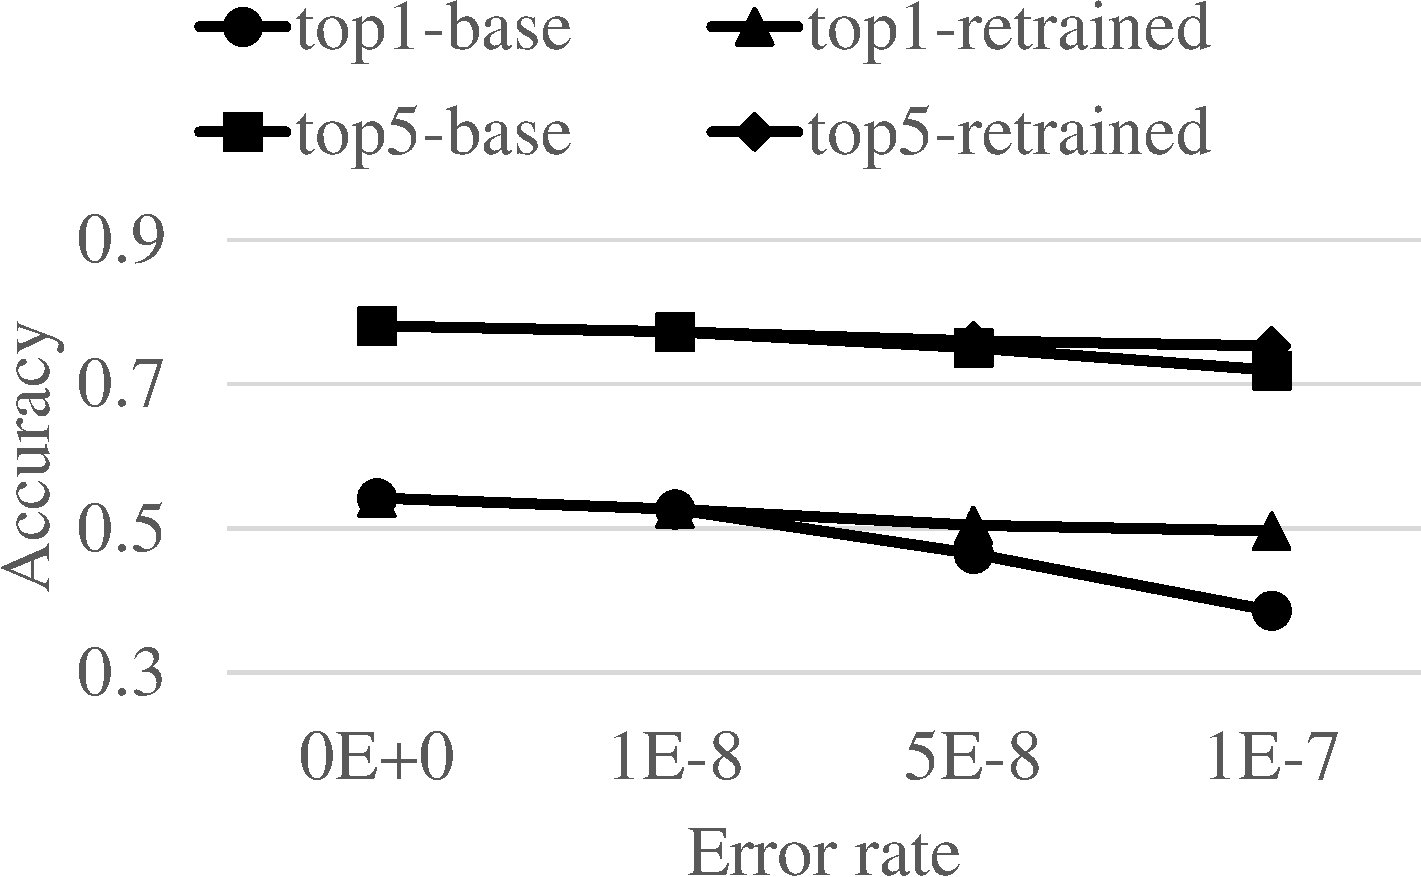
\includegraphics[width=0.7\linewidth]{alexnet-softerror}
        }
        \qquad
        \subfloat[VGG-16]{
                \label{fig:vgg16}
                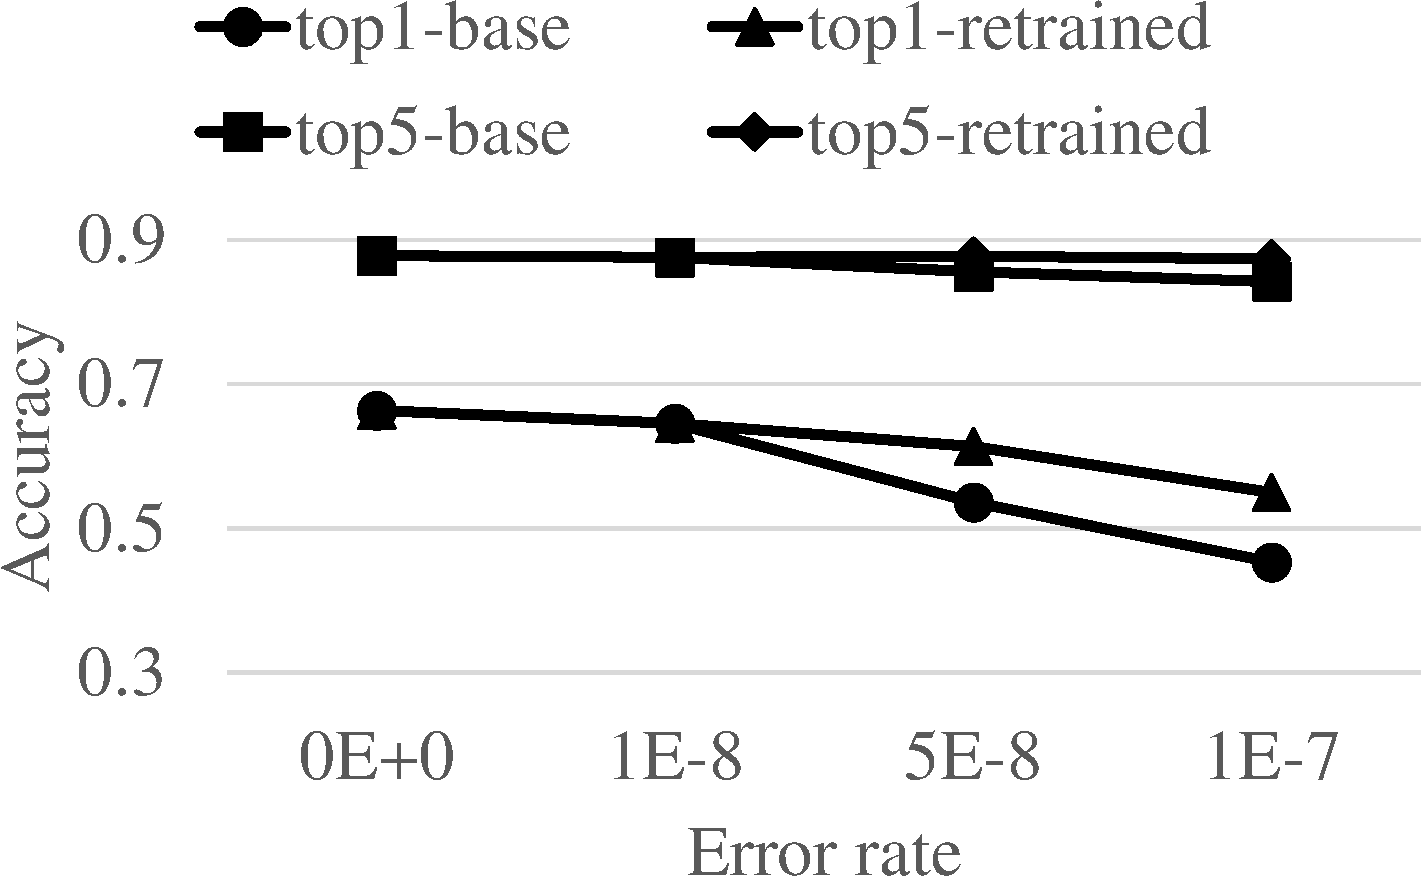
\includegraphics[width=0.7\linewidth]{vgg16-softerror}
        }
        \qquad
        \subfloat[VGG-19]{
                \label{fig:vgg19}
                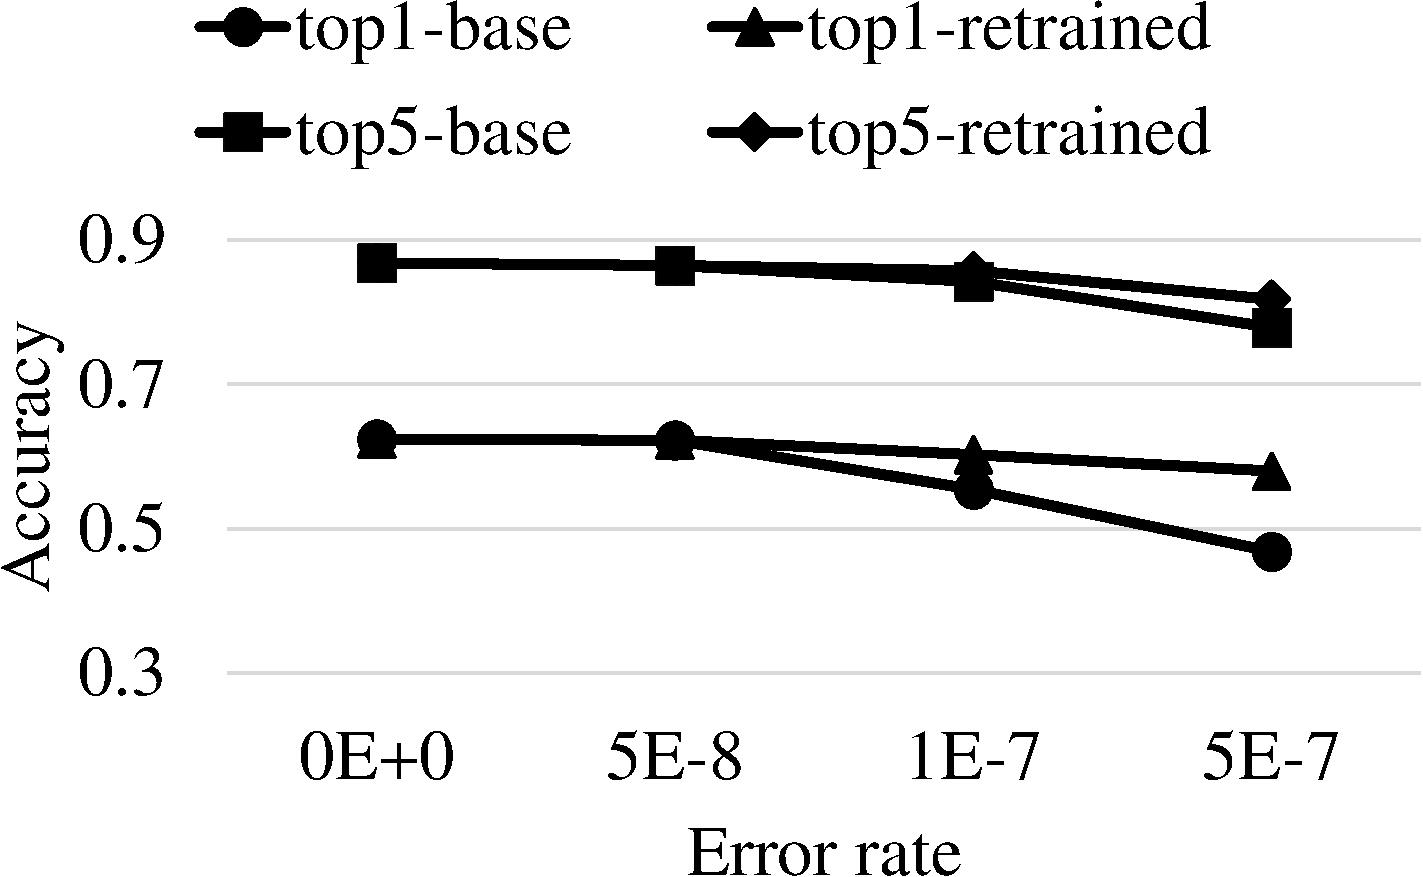
\includegraphics[width=0.7\linewidth]{vgg19-softerror}
        }
        \caption{The precision accuracy of the benchmark neural network models on accelerators with different computing errors}
        \label{fig:softerror-accuracy}
\end{figure}

\begin{figure}
        \center{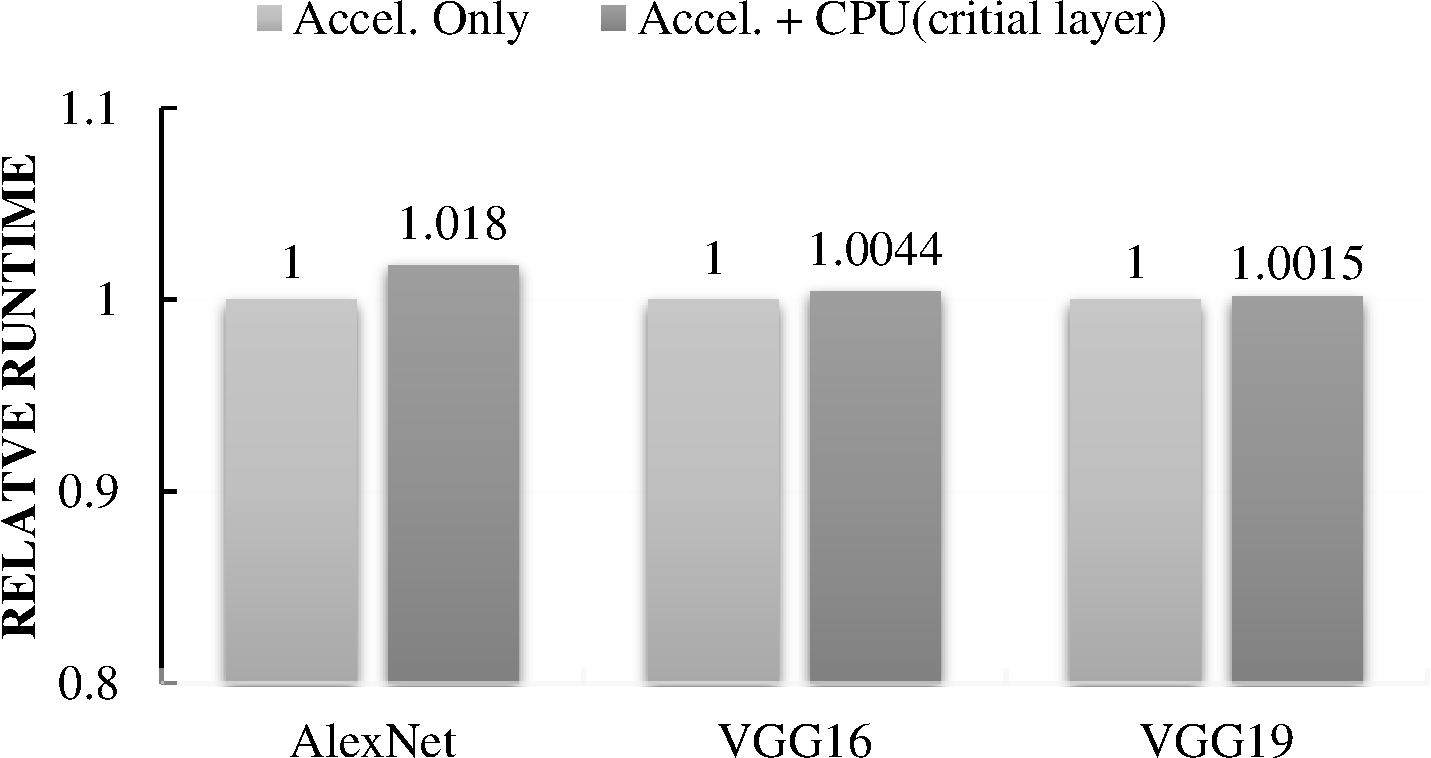
\includegraphics[width=0.7\linewidth]{clp_time}}
        \caption{Relative runtime of neural networks when the critical layer is scheduled to CPU.}
        \label{fig:clp_perf}
\end{figure}

We decide the critical layers using the error distribution as shown in Figure \ref{fig:clp_perf}.
We set the error threshold to be 5 and the experiment reveals that the last FC 
layer has the largest portion of computing errors that are more than 5. Thus, it is considered as 
the most critical layer. The critical layer takes only a small portion of the overall 
neural network computing, so the performance penalty is small even 
when it is scheduled to CPU. The last FC layer in AlexNet takes up higher portion of computing, 
the performance penalty is relatively higher compared to VGG16 and VGG19.
\begin{figure*}
        \center{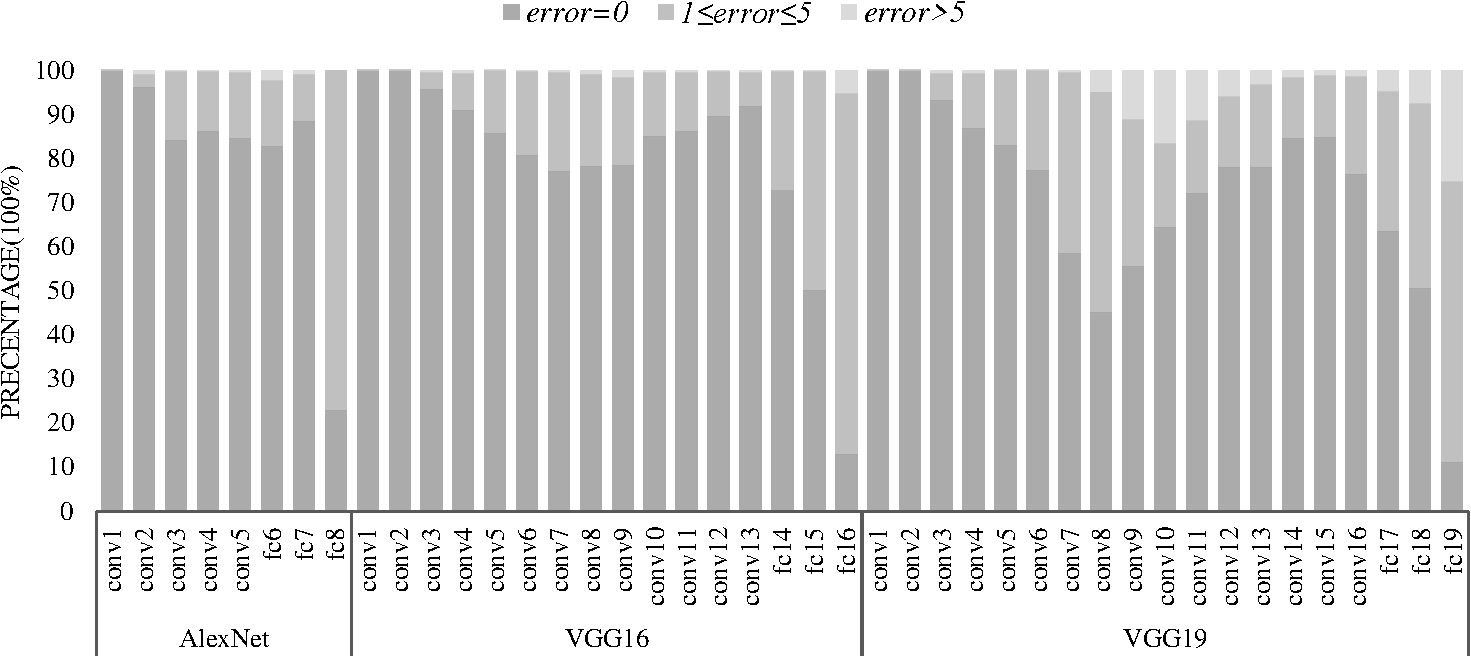
\includegraphics[width=0.8\linewidth]{error_distribute_softerror}}
        \caption{Error distribution across the neural network layers when highest BER is used in AlexNet, VGG16 and VGG19.}
        \label{fig:clp_perf}
\end{figure*}

\subsection{Overclocking case study}
To verify the proposed resilient training, we take overclocked CNN accelerator on KCU1500 as a case 
study in this work. By relaxing the timing constraints, the CNN accelerator can 
run at higher clock frequency with timing violations and computing errors. In PipeCNN, the 
hardware implementation is related to the neural network. For AlexNet, VGG16 and VGG19, the 
default implementation frequency is 210 MHz, 190 MHz and 190 MHz respectively. We then apply overclocking 
on the implementations with 10MHz step. The frequency can be boosted to 
260 MHz MHz, 240 MHz MHz and 240 MHz at most. By retraining the original neural network with 
the proposed approach, the prediction accuracy improvement is evaluated in detail.

With the overclocked CNN accelerators, we compare both the offline 
training and the proposed resilient training as presented in Figure \ref{fig:overclock-accuracy}. 
The prediction accuracy remains unchanged at the beginning and exhibits cliff-like drop 
at a tipping point. Beyond the tipping point, the prediction is no longer interesting 
due to the extremely low accuracy. At the tipping point, the top1 and top5 prediction accuracy of the 
retrained neural networks improves by xxx and xxx respectively.

\begin{figure}
        \center
	\subfloat[AlexNet]{
                \label{fig:alexnet}
                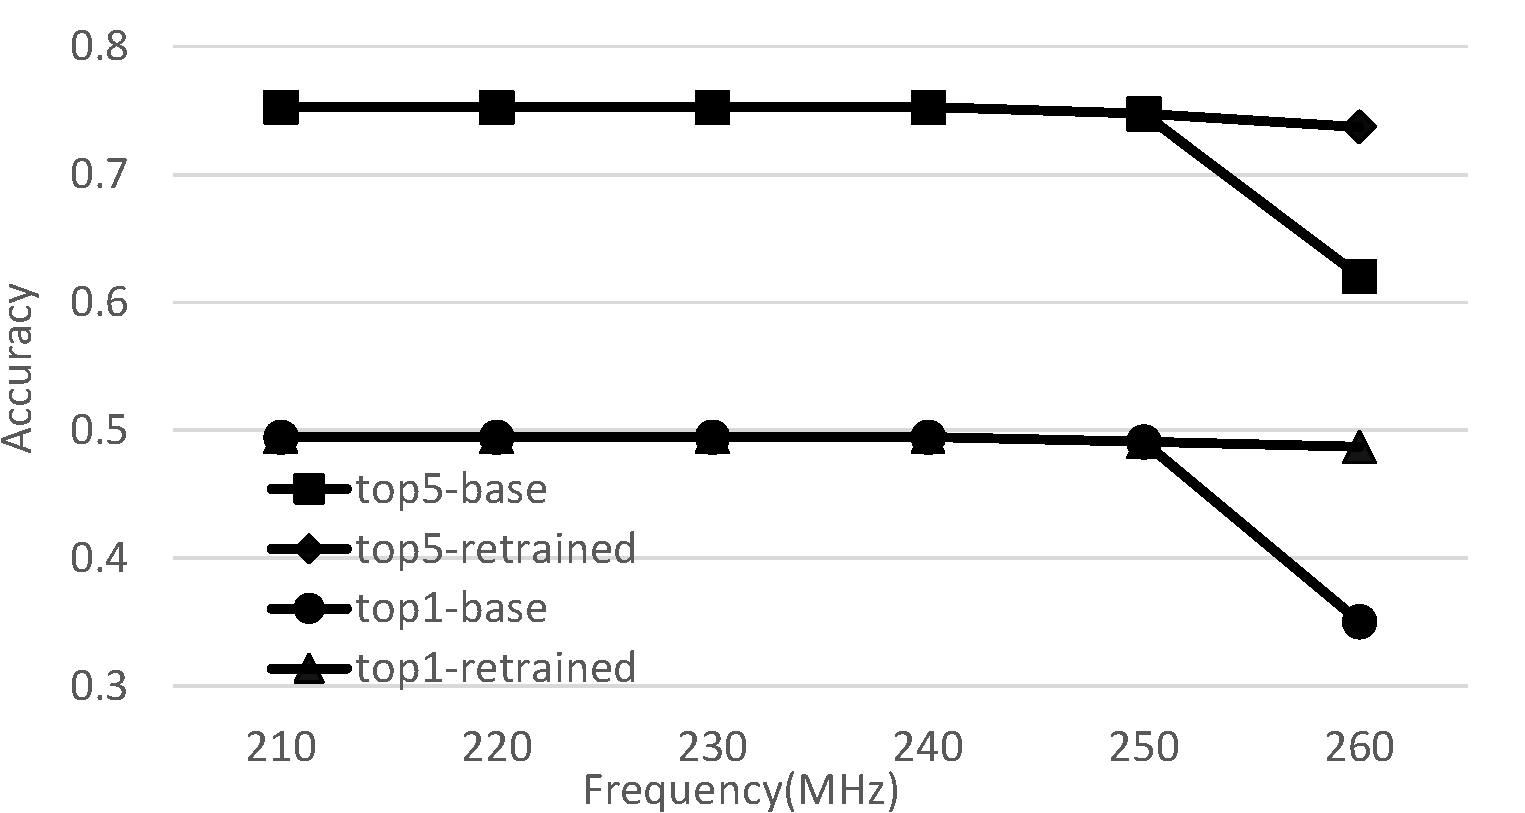
\includegraphics[width=0.6\linewidth]{alexnet-overclock}
        }
	\qquad
	\subfloat[VGG-16]{
                \label{fig:vgg16}
                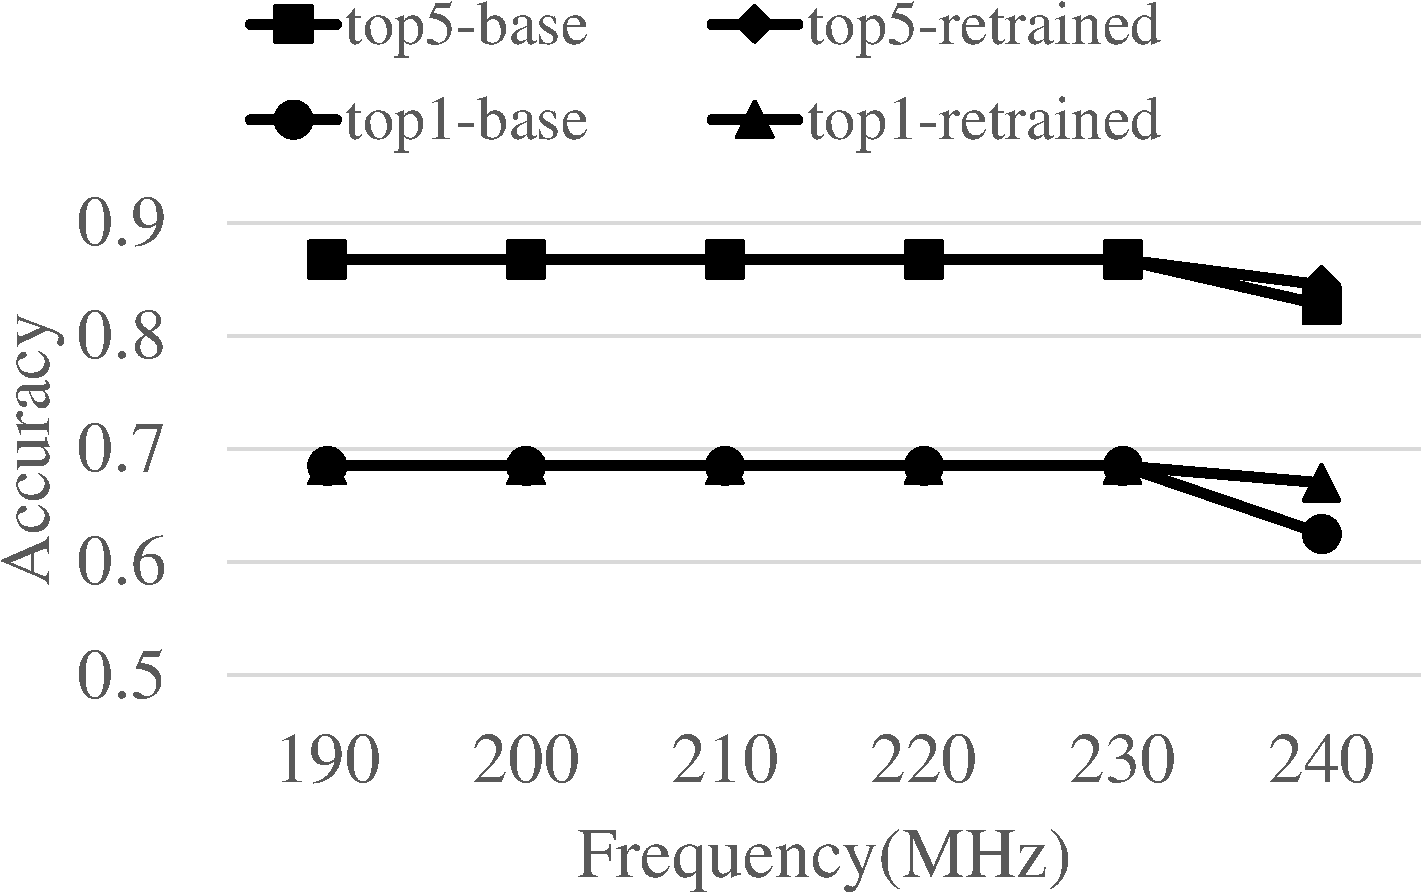
\includegraphics[width=0.6\linewidth]{vgg16-overclock}
        }
        \qquad
	\subfloat[VGG-19]{
                \label{fig:vgg19}
                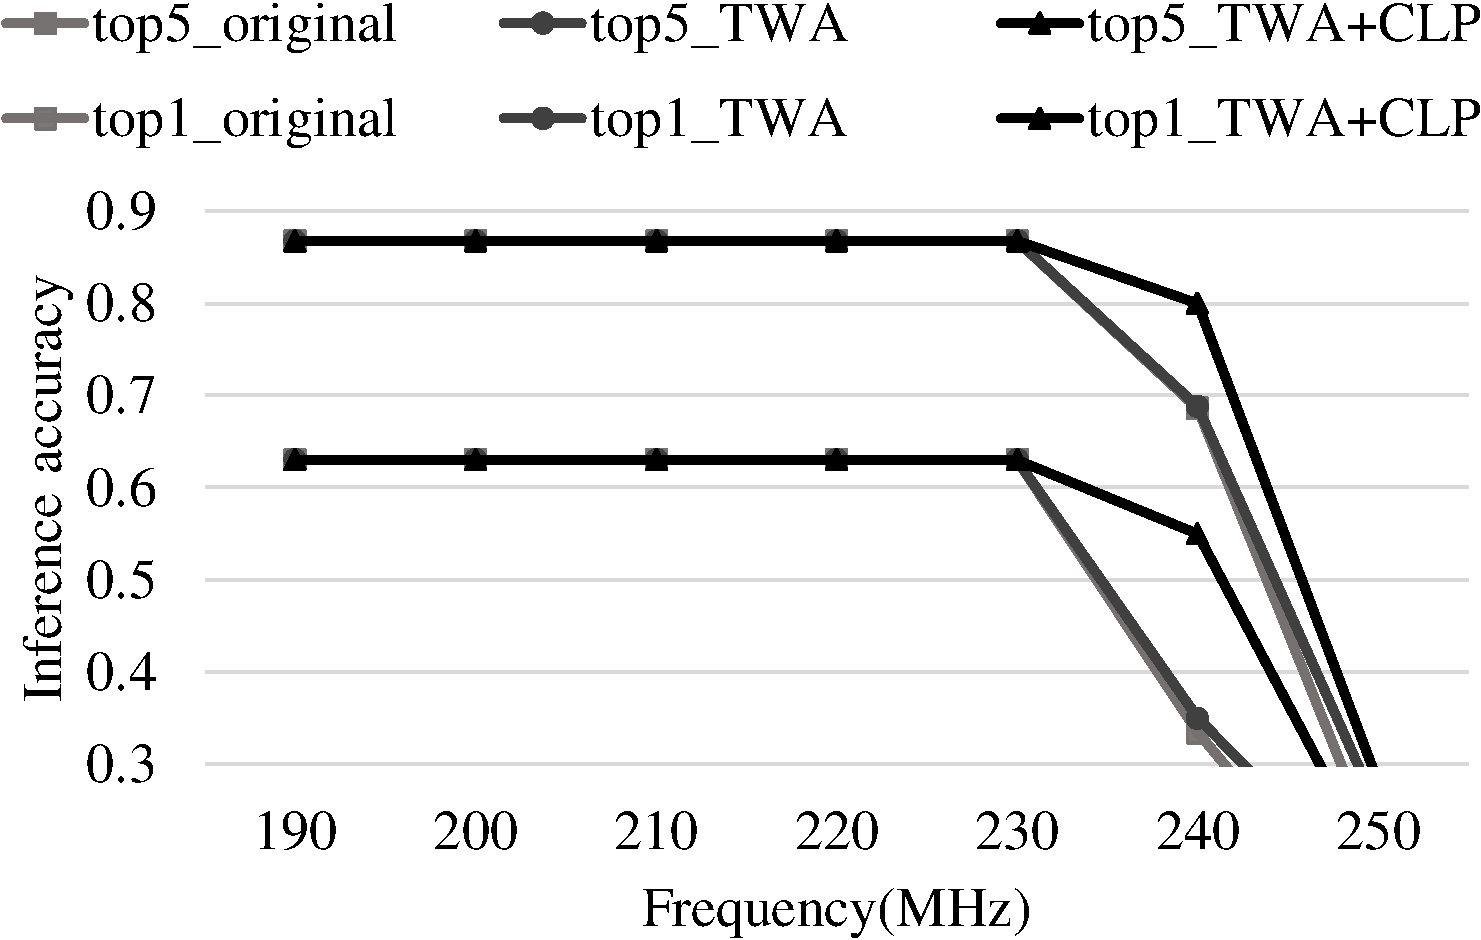
\includegraphics[width=0.6\linewidth]{vgg19-overclock}
        }
	\caption{The prediction accuracy of the benchmark neural networks on accelerators with different overclocking}
        \label{fig:overclock-accuracy}
\end{figure}

Clock frequency is almost proportional to the performance of the CNN accelerator 
especially for large convolution operation which is typically computing bound. 
Figure \ref{fig:overclocking-time} shows the relative inference runtime of the three neural networks at different 
overclocking. On the tipping point which is also the extreme overclocking case, 
the runtime improves by xxx compared to the models running on normal accelerator with 
xxx top1 accuracy loss and xxx top5 accuracy loss on average. 
\begin{figure}
        \center{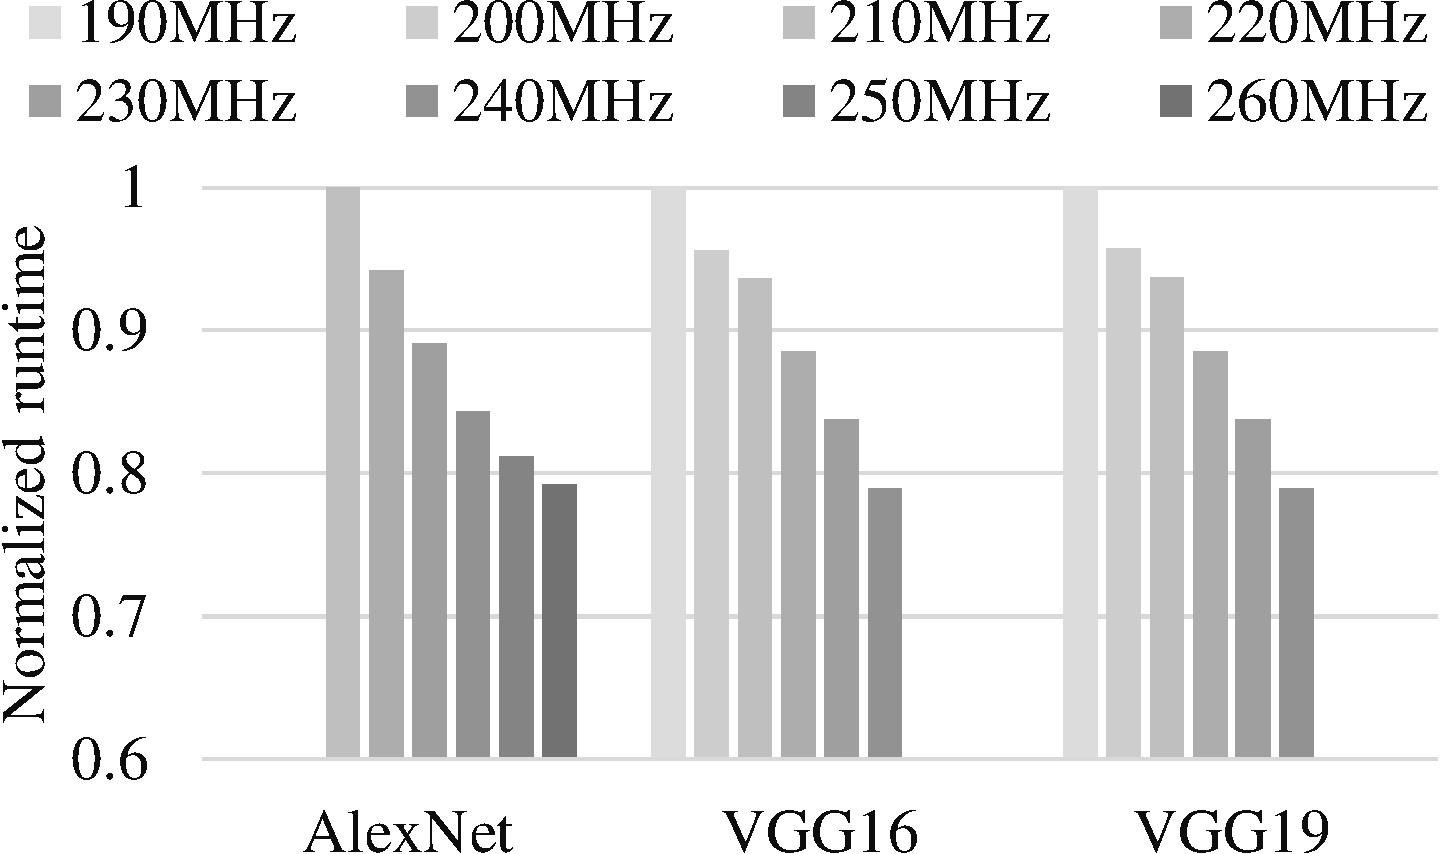
\includegraphics[width=0.6\linewidth]{relative-runtime}}
        \caption{Relative runtime of the neural networks on CNN accelerators with different overclocking. Note that AlexNet runs from 210 MHz to 250 MHz while 
		VGG16 and VGG19 ranges from 190 MHz to 240MHz, so some of the data is left blank.}
        \label{fig:overclocking-time}
\end{figure}

Comparing the experiments with random error simulation and overclocking on realistic FPGAs, we
find that the computing errors may not be uniformly distributed. In the overclocking,  
the prediction accuracy drops with cliff-like style. It indicates the computing errors may 
be quite small with light overclocking, but the amount of errors explodes at certain point.
Fortunately, the general trend is similar and the proposed training produces more resilient 
neural networks. 


